% Figure: traceable data-to-deployment loop.  An audit only means something if four
% facts are recorded: where a sample came from, how the split was made, which
% distribution it was evaluated on, and which generated samples were fed back.
% Design width ~168mm.
\documentclass[border=0pt]{standalone}
\usepackage{amsmath,amssymb}
% Shared visual language for the figures of the book.
% Every figure in this directory loads this file so the chapter reads as one system.
% NOTE: no blank lines are allowed inside \tikzset{...} (a blank line emits \par
% and breaks key scanning).
\NeedsTeXFormat{LaTeX2e}
\ProvidesPackage{figstyle}[2026/10/21 Figure style for Free Energy to LLMs]

\RequirePackage{tikz}
\usetikzlibrary{arrows.meta,positioning,calc,fit,shapes.geometric,shapes.misc,%
  backgrounds,matrix,decorations.pathreplacing,decorations.markings,patterns.meta}

% ---------------------------------------------------------------- palette
% Same values as book/preamble/style.tex, prefixed with F.
\definecolor{FNavy}{HTML}{14324A}
\definecolor{FTeal}{HTML}{0E7490}
\definecolor{FSky}{HTML}{E7F5F8}
\definecolor{FOrange}{HTML}{D97706}
\definecolor{FAmber}{HTML}{FFF3D6}
\definecolor{FInk}{HTML}{1F2937}
\definecolor{FSlate}{HTML}{64748B}
\definecolor{FMist}{HTML}{F5F7FA}
\definecolor{FRose}{HTML}{9F1239}
\definecolor{FRoseMist}{HTML}{FFF1F2}

% ---------------------------------------------------------------- semantics
% Teal   = probability / model / data object
% Orange = training objective, cost, or the quantity moved through the system
% Navy   = neutral structure
% Slate  = secondary label or metadata
% Rose   = failure mode, hazard, masked-out region
\tikzset{
  % Lay figures out in millimetres.  A figure designed 168mm wide is included at
  % \textwidth, so its fonts appear at exactly the size written here.
  every picture/.style={x=1mm,y=1mm,font=\small,line cap=round,line join=round},
  % ---- block styles
  nbase/.style={draw,rounded corners=1.2pt,align=center,inner sep=2.4pt,%
    minimum height=7mm,text=FInk},
  nteal/.style={nbase,draw=FTeal,fill=FSky},
  norange/.style={nbase,draw=FOrange,fill=FAmber},
  nnavy/.style={nbase,draw=FNavy,fill=white},
  nsoft/.style={nbase,draw=FSlate!55,fill=FMist},
  nrose/.style={nbase,draw=FRose,fill=FRoseMist},
  ghost/.style={draw=none,fill=none,align=center,inner sep=1pt},
  plain/.style={draw=none,fill=none,align=center,inner sep=0pt},
  % ---- arrows
  ar/.style={-{Latex[length=1.7mm,width=1.35mm]},draw=FSlate,line width=0.75pt},
  ard/.style={ar,dashed},
  arteal/.style={ar,draw=FTeal},
  arorange/.style={ar,draw=FOrange},
  arrose/.style={ar,draw=FRose},
  thickar/.style={ar,line width=1.2pt},
  % ---- text roles
  ftitle/.style={font=\large\bfseries,text=FNavy,align=center},
  ptitle/.style={font=\small\bfseries,text=FNavy,align=center},
  ptitleo/.style={font=\small\bfseries,text=FOrange,align=center},
  lbl/.style={font=\scriptsize,text=FSlate,align=center,inner sep=1pt},
  lblt/.style={lbl,text=FTeal},
  lblo/.style={lbl,text=FOrange},
  lbln/.style={lbl,text=FNavy},
  lblr/.style={lbl,text=FRose},
  sub/.style={font=\scriptsize,text=FSlate!90,align=center,inner sep=1pt},
  monob/.style={font=\ttfamily\scriptsize,text=FInk,inner sep=1pt},
  mathb/.style={font=\small,text=FInk,inner sep=1pt},
  eqn/.style={font=\scriptsize,inner sep=1.5pt,text=FInk},
  % ---- decorations
  brace/.style={decorate,decoration={brace,amplitude=2.4pt},draw=FSlate,%
    line width=0.6pt},
  bracet/.style={brace,draw=FTeal},
  braceo/.style={brace,draw=FOrange},
  axis/.style={draw=FSlate!55,line width=0.6pt},
  guide/.style={draw=FSlate!45,line width=0.5pt,dashed},
  halolabel/.style={font=\scriptsize,text=FInk,fill=white,fill opacity=0.85,%
    text opacity=1,inner sep=1.4pt,align=center},
}

% Figure title above the drawing, anchored at the figure's top-left.
\newcommand{\figtitle}[2][0]{%
  \node[ftitle,anchor=north west,outer sep=0pt] at (#1,0) {#2};}

% Rounded panel behind a subgroup of nodes.
\newcommand{\figpanel}[3][]{%
  \node[draw=FSlate!35,fill=#3,rounded corners=2pt,inner sep=2.6mm,#1] {#2};}

\endinput

\begin{document}
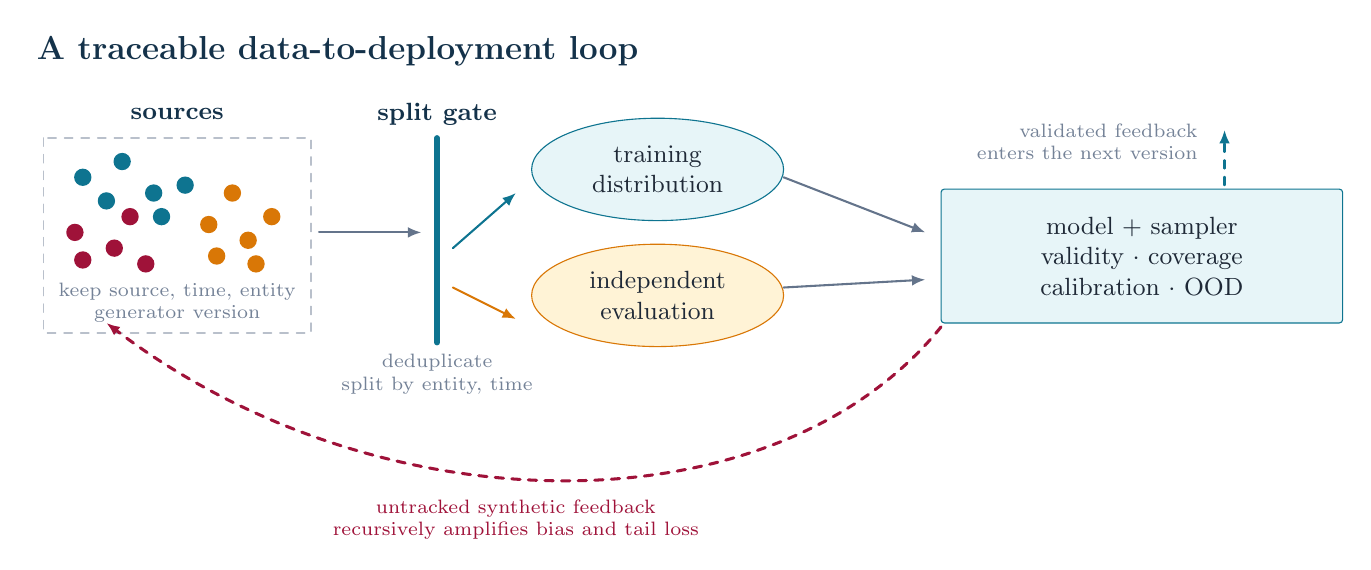
\begin{tikzpicture}
\figtitle{A traceable data-to-deployment loop}
% ------------------------------------------------------------------ band labels
\node[ptitle] at (19,-11) {sources};
\node[ptitle] at (52,-11) {split gate};
% ---------------------------------------------------------------------- sources
\draw[guide,dashed] (2,-14) rectangle (36,-38.8);
\foreach \x/\y in {7/-19,12/-17,16/-21,10/-22,20/-20,17/-24}
  {\fill[FTeal] (\x,\y) circle (1.1);}
\foreach \x/\y in {23/-25,28/-27,26/-21,31/-24,29/-30,24/-29}
  {\fill[FOrange] (\x,\y) circle (1.1);}
\foreach \x/\y in {6/-26,11/-28,15/-30,7/-29.5,13/-24}
  {\fill[FRose] (\x,\y) circle (1.1);}
\node[sub] at (19,-33.5) {keep source, time, entity};
\node[sub] at (19,-36.4) {generator version};
\draw[ar] (37,-26)--(50,-26);
% --------------------------------------------------------------------- split gate
\draw[FTeal,line width=2pt] (52,-14)--(52,-40);
\node[sub] at (52,-44) {deduplicate\\split by entity, time};
% ------------------------------------------------------- training and evaluation
\draw[arteal] (54,-28)--(62,-21);
\draw[arorange] (54,-33)--(62,-37);
\node[draw=FTeal,fill=FSky,ellipse,minimum width=32mm,minimum height=13mm,%
  align=center,text=FInk] at (80,-18) {training\\distribution};
\node[draw=FOrange,fill=FAmber,ellipse,minimum width=32mm,minimum height=13mm,%
  align=center,text=FInk] at (80,-34) {independent\\evaluation};
\draw[ar] (96,-19)--(114,-26);
\draw[ar] (96,-33)--(114,-32);
% --------------------------------------------------------------- model + sampler
\node[nteal,minimum width=51mm,minimum height=17mm,align=center] at (141.5,-29)
  {model $+$ sampler\\validity $\cdot$ coverage\\calibration $\cdot$ OOD};
\draw[arteal,dashed] (152,-20)--(152,-13);
\node[sub,anchor=east,align=right] at (149,-14.5)
  {validated feedback\\enters the next version};
% --------------------------------------------------------------- feedback paths
\draw[arrose,dashed,line width=1.1pt] (116,-38) .. controls (95,-64) and (45,-64) .. (10,-37.5);
\node[lblr] at (62,-62.5)
  {untracked synthetic feedback\\recursively amplifies bias and tail loss};
\end{tikzpicture}
\end{document}
